\chapter{An Ensemble Detector}
\label{ch:ensemble}

\section{From One Detector to Many}

Chapter~3 ended on a diagnosis: ReReReRe is a strong detector of
\emph{inconsistent} careless responding but is, by design, nearly blind to
\emph{consistent} patterns such as straightlining and acquiescence, weak at low
dimensionality, and---like any single index---limited by the need to commit to
one threshold. Each of these limits is the mirror image of a strength of some
other detector. Longstring and low intra-individual variability catch
straightliners outright; Mahalanobis distance catches multivariate outliers.
The detectors are \emph{complementary}: they fail on different respondents.

This chapter turns that complementarity into a single, better detector. Rather
than choosing one index or applying several under separate ad hoc cutoffs---the
informal multi-index practice that Chapter~1 described as the field's de facto
recommendation \parencite{curran2016methods, ward2023dealing}---it treats each
index as one \emph{feature} and lets a trained classifier learn how to weigh
them and when to trust each. The classifier is a Random Forest
\parencite{breiman2001random}, and the central empirical question of the chapter
is whether ReReReRe contributes anything \emph{beyond} the established
auxiliary detectors, and if so, how much and under what conditions. The answer,
developed with bootstrap confidence intervals, is that its contribution is
statistically positive at every questionnaire length and grows substantially
with length.

\section{The Five Features}

Each respondent is summarized by five detector scores, all oriented so that
\emph{higher means more careless}:

\begin{quote}
\small
\begin{description}\setlength{\itemsep}{2pt}
\item[$z_{\text{RR}}$] the ReReReRe permutation coherence z-score of Chapter~3,
  sign-flipped so that low coherence (incoherent, inconsistent careless) reads
  as a high feature value.
\item[IRV] the (negated) intra-individual response variability
  \parencite{dunn2018intra}: low dispersion---the signature of
  straightlining---reads as high careless.
\item[LongString] the longest run of identical consecutive responses
  \parencite{johnson2005ascertaining}.
\item[$D^2$] the Mahalanobis distance from the sample centroid
  \parencite{mahalanobis1936generalised}: multivariate outlyingness.
\item[Person--Total] the (negated) correlation between a respondent's profile
  and the sample mean profile: answering against the grain.
\end{description}
\end{quote}

The first feature is the contribution of this thesis; the remaining four are the
established indices reviewed in Chapter~1. The design intention is explicit
division of labour: ReReReRe carries the \emph{inconsistent}-careless signal that
the four auxiliaries miss, while the auxiliaries carry the \emph{consistent}
signal that ReReReRe misses. Whether that intention is realized is tested in
Section~4.6.

\section{The Random Forest Combiner}

The five features are combined by a Random Forest (Section~\ref{sec:rf}): an ensemble of
200 decision trees, each grown on a bootstrap resample of the training
respondents, each split considering a random subset of the features, the final
predicted careless probability being the proportion of trees voting
``careless.'' Two properties make the Random Forest the right combiner here.
First, the features interact: a respondent with both a low $z_{\text{RR}}$
\emph{and} a low IRV is far more suspicious than the additive combination of the
two signals implies, because that conjunction is the signature of a
straightliner who also breaks cross-factor coherence. Trees capture such
interactions automatically. Second, the Random Forest is robust to features on
different scales and to redundancy among them, so the five detectors can be fed
in raw. In our simulations the Random Forest outperformed logistic regression
and elastic-net regression on every evaluation metric considered, with the
widest margins on the hardest conditions (short questionnaires and low base
rates), consistent with the non-linear, interactive structure of the problem.

Throughout, the classifier is evaluated by five-fold cross-validation
(Section~\ref{sec:cv}): each respondent receives an out-of-fold predicted probability
from a forest that did not see them in training, and these out-of-fold
predictions are used for every metric reported below. This guards against the
optimism that would arise from scoring the classifier on its own training data.

\section{Operational Definition of Careless}

Evaluating a detector requires a ground-truth label, and in simulated data a
respondent's corruption can be set to any degree. We therefore need an explicit
rule for \emph{how corrupted} a respondent must be to count as careless. This
rule is not innocuous: set it too high and the negative class is contaminated
with heavily corrupted respondents; set it too low and trivially-corrupted
respondents inflate the positive class.

We fix the rule empirically. A respondent is labelled careless when the
corrupted fraction of their row exceeds $\tau = 0.40$, and \emph{every} other
respondent---clean and lightly corrupted alike---stays in the negative class.
The cutoff $\tau = 0.40$ is the joint argmax of the Matthews correlation
coefficient, Cohen's $\kappa$, Youden's J, and balanced accuracy across a sweep
$\tau \in \{0.10, 0.20, \dots, 0.90\}$ evaluated on 24{,}000 simulated
respondents. (Two secondary metrics, F1 and AUPRC, favour slightly lower cutoffs
of $0.30$ and $0.20$; the four primary classification metrics agree unanimously
on $0.40$.) Crucially, this is the \emph{deployment-realistic} framing: in real
data the analyst does not know in advance who has 30\% versus 60\% corruption, so
keeping the lightly-corrupted respondents in the negative class tests whether the
detector recovers moderately-to-fully corrupted rows without false-flagging the
ambiguous middle. An earlier, looser definition that excluded the middle from
the negative class was discarded as artificially easy.

\section{Simulation Design and Headline Performance}

The ensemble was evaluated on a simulation grid of \textbf{384 datasets}
crossing eight questionnaire sizes (30, 50, 80, 100, 150, 200, 250, and 300
items), four careless base rates (10\%, 20\%, 40\%, 60\%), and twelve
replications per cell, with $n = 500$ respondents each. Within every dataset,
careless respondents were injected at one of six prototypical patterns---random,
longstring, mixed, fatigue, acquiescent, pure straightlining---with the
corrupted fraction drawn from $\{0\%, 10\%, \dots, 100\%\}$, so that the full
corruption continuum is represented. The five features were computed for every
respondent and a Random Forest trained under five-fold cross-validation.

The operating point is set by the \emph{rate-aware} calibration, the deployable
rule developed in Chapter~5: the analyst supplies a rough prior on the careless
base rate and the threshold is placed at the corresponding quantile of the
predicted probabilities, requiring no labels. Pooled across all sizes and rates,
the ensemble reaches the performance in Table~\ref{tab:headline}.

\begin{table}[t]
\centering
\caption{Pooled detection performance of the five-feature ensemble under the
rate-aware operating point (160 cells, five-fold CV within each).}
\label{tab:headline}
\small
\begin{tabular}{l c}
\toprule
\textbf{Metric} & \textbf{Pooled value} \\
\midrule
MCC          & 0.662 \\
F1           & 0.730 \\
Sensitivity  & 0.731 \\
Specificity  & 0.932 \\
AUC          & 0.919 \\
\bottomrule
\end{tabular}
\end{table}

Detection quality scales smoothly with questionnaire length
(Table~\ref{tab:scaling}). At 30 items the ensemble is useful but modest
(MCC $= 0.44$); by 150 items it is strong (MCC $= 0.72$); and it approaches its
asymptote near 300 items (MCC $= 0.82$), where the $250 \rightarrow 300$ gain is
only $+0.017$. This is the same total-length scaling identified for ReReReRe
alone in Chapter~3, now inherited by the ensemble.

\begin{table}[t]
\centering
\caption{Per-size detection (MCC) under the rate-aware operating point.}
\label{tab:scaling}
\small
\begin{tabular}{l c c c c c c c c}
\toprule
\textbf{Items} & 30 & 50 & 80 & 100 & 150 & 200 & 250 & 300 \\
\midrule
\textbf{MCC} & 0.439 & 0.525 & 0.604 & 0.630 & 0.717 & 0.771 & 0.798 & 0.815 \\
\bottomrule
\end{tabular}
\end{table}

\section{The Contribution of ReReReRe}

The chapter's central question is whether ReReReRe earns its place in the
ensemble. We answer it by \emph{ablation}: training the same Random Forest under
two feature sets---the full five features, and the four auxiliaries only---and
comparing them under the identical cross-validation protocol and operational
definition.

\subsection{Ablation by questionnaire length}

Figure~\ref{fig:ablation} shows the two configurations as a function of
questionnaire length. The full ensemble (with ReReReRe) rises from MCC
$\approx 0.42$ at 30 items to $\approx 0.74$ at 300; the auxiliaries-only
ensemble rises from $\approx 0.40$ to only $\approx 0.61$ and then plateaus. The
gap between the curves \emph{widens monotonically} with length: at short
questionnaires the four auxiliaries already capture most of the available
signal, but at long questionnaires they saturate while the full ensemble keeps
improving. Adding more auxiliary detectors does not close this gap---it is
specifically the cross-factor coherence signal, available only from ReReReRe,
that the auxiliaries cannot supply.

\begin{figure}[t]
\centering
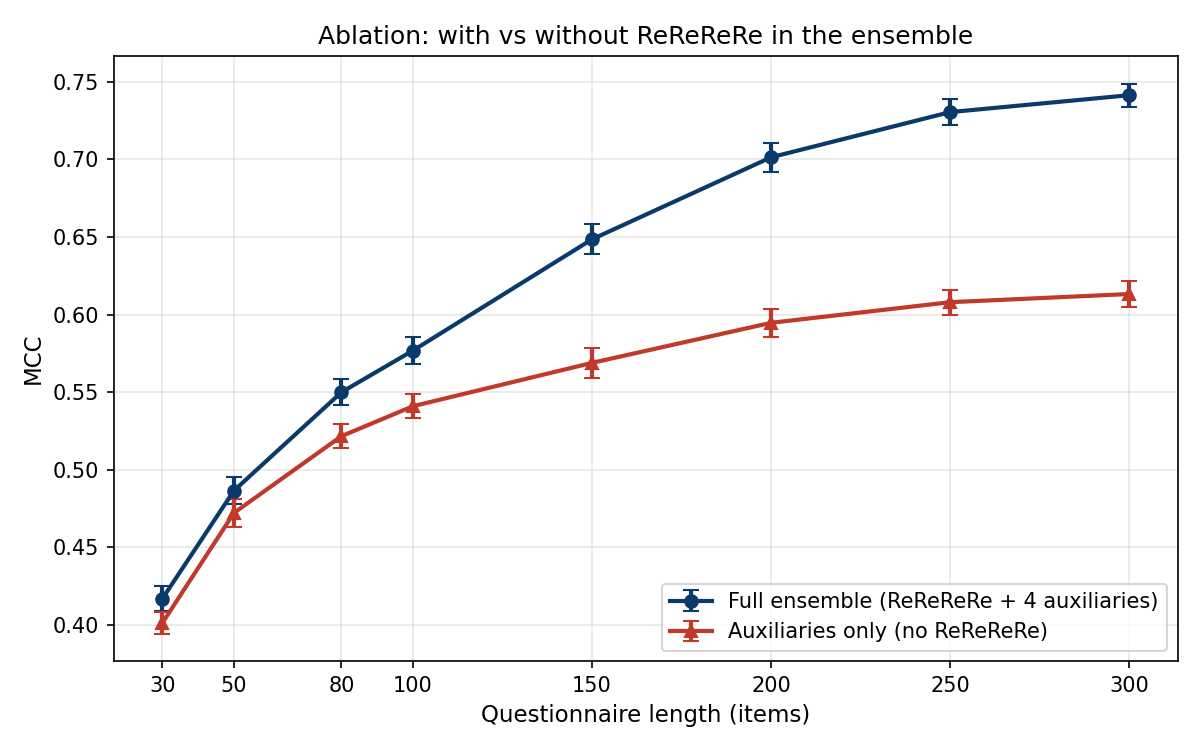
\includegraphics[width=0.95\linewidth]{figures/fig_ensemble_ablation.png}
\caption{Ablation by questionnaire length. The full five-feature ensemble
(ReReReRe + four auxiliaries) versus the four auxiliaries alone, both trained
under five-fold cross-validation with the same operational definition. Error
bars are $\pm 1$ SEM. The gap grows from a small margin at 30 items to a sizeable
one at 200--300 items.}
\label{fig:ablation}
\end{figure}

\subsection{Bootstrap confidence intervals on the contribution}

A difference of curves is suggestive; to make the claim inferential we put a
confidence interval on it. For each questionnaire size we bootstrapped over
respondent indices (500 resamples; Section~\ref{sec:boot}) and recomputed
$\Delta\text{MCC} = \text{MCC(full)} - \text{MCC(auxiliaries only)}$ on each
resample, taking the 2.5th and 97.5th percentiles as a 95\% interval.
Table~\ref{tab:delta} and Figure~\ref{fig:delta} report the result.

\begin{table}[t]
\centering
\caption{Bootstrap 95\% confidence intervals on the contribution of ReReReRe,
$\Delta\text{MCC} = \text{MCC(full)} - \text{MCC(auxiliaries only)}$, by
questionnaire length.}
\label{tab:delta}
\small
\begin{tabular}{l c c c}
\toprule
\textbf{Items} & \textbf{$\Delta$MCC} & \textbf{95\% CI} & \textbf{$P(\Delta>0)$} \\
\midrule
30  & $+0.020$ & $[+0.009,\ +0.031]$ & 1.000 \\
50  & $+0.018$ & $[+0.008,\ +0.028]$ & 1.000 \\
80  & $+0.035$ & $[+0.024,\ +0.046]$ & 1.000 \\
100 & $+0.035$ & $[+0.025,\ +0.045]$ & 1.000 \\
150 & $+0.096$ & $[+0.085,\ +0.110]$ & 1.000 \\
200 & $+0.121$ & $[+0.108,\ +0.133]$ & 1.000 \\
250 & $+0.133$ & $[+0.120,\ +0.145]$ & 1.000 \\
300 & $+0.150$ & $[+0.138,\ +0.163]$ & 1.000 \\
\bottomrule
\end{tabular}
\end{table}

\begin{figure}[t]
\centering
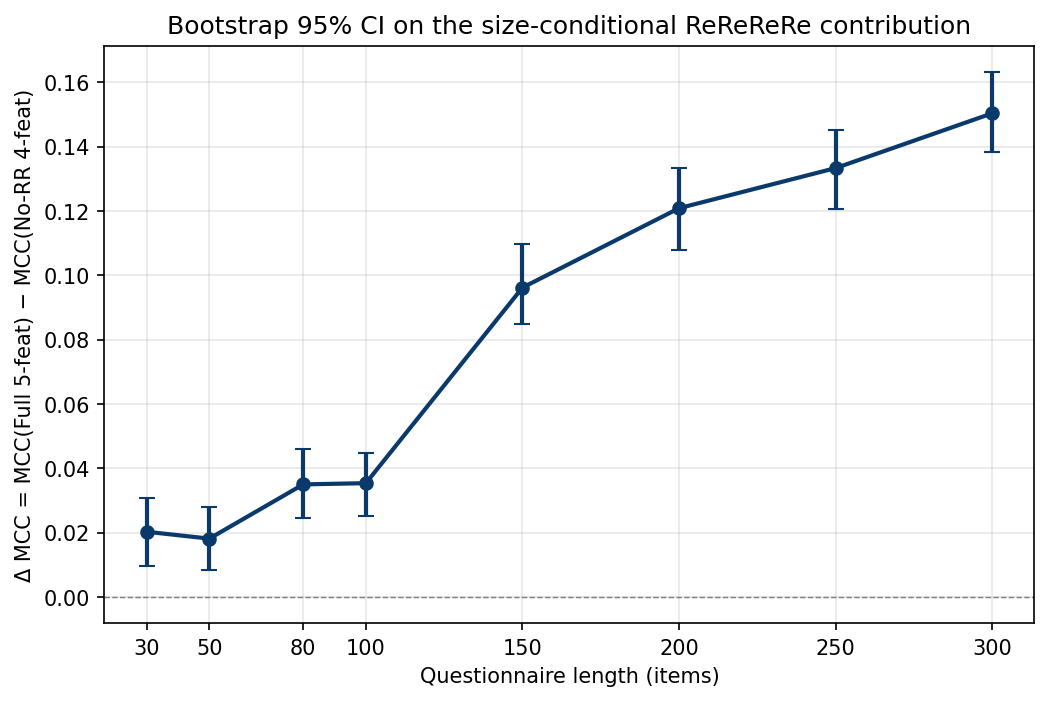
\includegraphics[width=0.85\linewidth]{figures/fig_bootstrap_delta.png}
\caption{Bootstrap 95\% confidence interval on the size-conditional contribution
of ReReReRe ($\Delta$MCC = full $-$ auxiliaries only). The interval excludes zero
at every questionnaire length; the contribution grows from $+0.020$ at 30 items
to $+0.150$ at 300 items.}
\label{fig:delta}
\end{figure}

The interval \emph{excludes zero at every size tested}, so the contribution of
ReReReRe is statistically positive throughout---including the 30-item case, where
one might have expected it to be redundant. The \emph{magnitude}, however, is
strongly length-dependent: small below 100 items ($\approx +0.02$ to $+0.035$)
and large above 150 items ($+0.10$ to $+0.15$, roughly a quarter of the
auxiliaries' ceiling). This is the chapter's headline structural finding, and it
has a clear practical reading: ReReReRe pays off most on the long
multi-construct batteries that dominate modern psychometric practice
(150--300 items), not on the short unidimensional scales where it would be
easiest to dismiss as redundant.

\section{Where the Contribution Comes From}

The ablation says \emph{how much} ReReReRe contributes; the per-pattern
breakdown says \emph{where}. Figure~\ref{fig:pattern} plots detection rate
against corruption fraction for each of the six injected patterns, comparing the
full ensemble with the auxiliaries-only ensemble.

\begin{figure}[t]
\centering
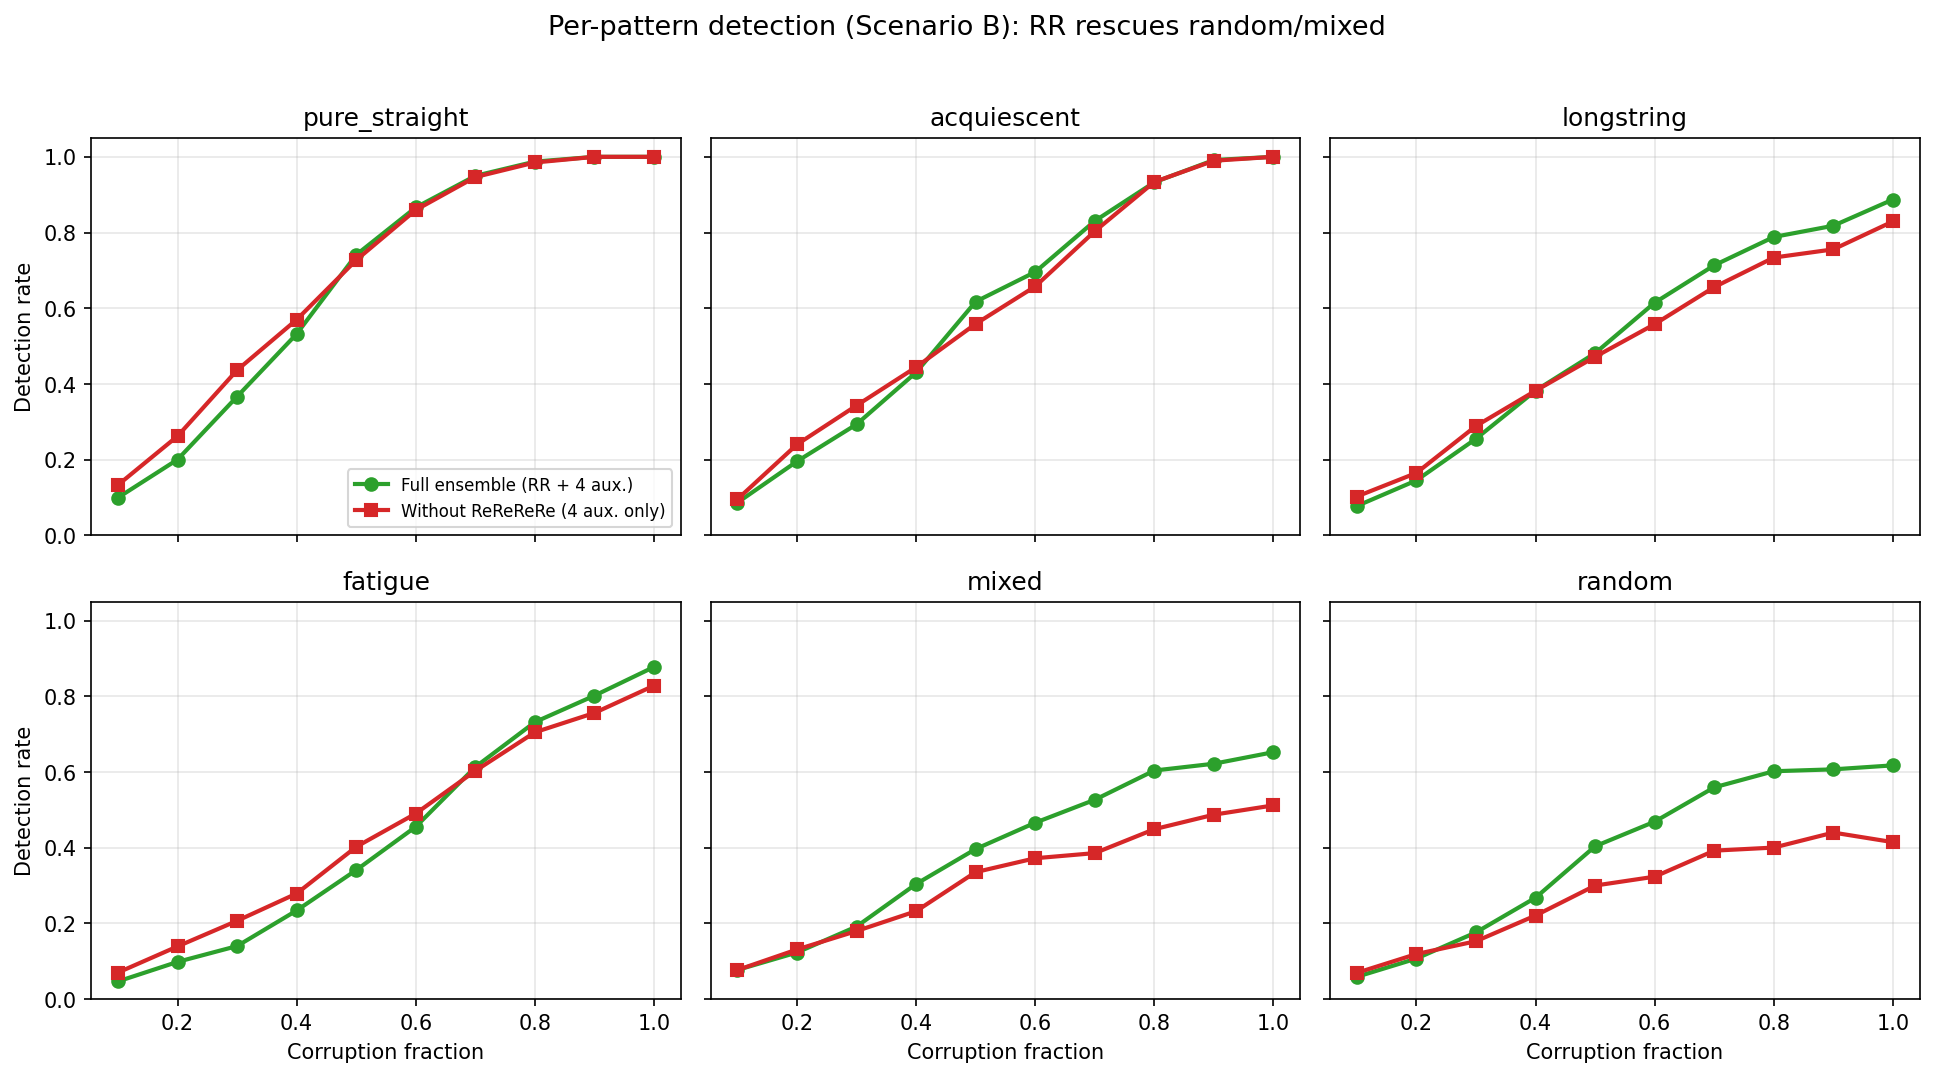
\includegraphics[width=0.98\linewidth]{figures/fig_per_pattern.png}
\caption{Per-pattern detection: full ensemble (green) versus auxiliaries only
(red), by corruption fraction. The two coincide on consistent patterns
(pure straightlining, acquiescence, longstring, fatigue), which the auxiliaries
already detect; they diverge on the inconsistent patterns (mixed, random), where
ReReReRe supplies the signal the auxiliaries lack.}
\label{fig:pattern}
\end{figure}

The picture is exactly the complementarity the ensemble was designed to exploit.
On the \emph{consistent} patterns---pure straightlining, acquiescence, and
highly-corrupted longstring and fatigue---the two curves are essentially
identical: the auxiliary detectors already saturate, and ReReReRe adds nothing,
because a respondent who selects the same option throughout is trivially caught
by LongString and low IRV. On the \emph{inconsistent} patterns---mixed and,
especially, random---the full ensemble (green) sits well above the
auxiliaries-only ensemble (red) across the whole corruption range: here the
auxiliaries are partly blind, and ReReReRe rescues respondents they miss. The
ensemble works not because every detector helps everywhere, but because the
detectors fail on disjoint sets of respondents, and the Random Forest learns to
route each case to whichever feature is informative for it.

\section{Summary}

Combining ReReReRe with four established auxiliary detectors inside a Random
Forest yields a single careless-detection model whose pooled performance
(MCC $= 0.66$, AUC $= 0.92$) scales from MCC $= 0.44$ on 30-item questionnaires
to MCC $= 0.82$ on 300-item batteries under a deployable, label-free operating
point. Ablation with bootstrap confidence intervals establishes that the
contribution of ReReReRe is statistically positive at every questionnaire length
and grows from $+0.02$ MCC on short instruments to $+0.15$ MCC on long ones. The
mechanism is complementarity: ReReReRe rescues the inconsistent careless patterns
(random, mixed) on which the auxiliary detectors are weak, while contributing
little on the consistent patterns they already catch. What remains is the
question the headline numbers quietly presupposed---how to set the operating
point \emph{without} the ground-truth labels that the cross-validation here had
access to. That is the deployment problem, and it is the subject of Chapter~5.

